\documentclass{article}
\usepackage[T1]{fontenc}
\usepackage{lmodern}
\usepackage{graphicx}
\usepackage{amsmath,amssymb}
\usepackage[a4paper,margin=2cm]{geometry}
\usepackage[absolute,overlay]{textpos}
\setlength{\TPHorizModule}{1mm}
\setlength{\TPVertModule}{1mm}
\usepackage[indonesian]{babel}
\usepackage{hyperref}
\setlength{\emergencystretch}{2em}
% unit: Halaman 8

\begin{document}

% === Halaman 8 (llm) ===

\vspace{238.79mm}

Ingat kembali stegosploit!!!

\vspace{10mm}

Just look at the image and you are HACKED!

\url{http://thehackernews.com/2015/06/Stegosploit-malware.html}

% deskripsi: Screenshot artikel berita tentang Stegosploit yang menunjukkan gambar kucing dengan teks overlay 'THIS PICTURE CAN HACK YOUR COMPUTER' dan penjelasan mengenai teknik menyembunyikan kode berbahaya dalam piksel gambar.
% bbox normalisasi: [0.0600, 0.1080, 0.9400, 0.9120]
\begin{textblock*}{184.80mm}(12.60mm,32.08mm)
\noindent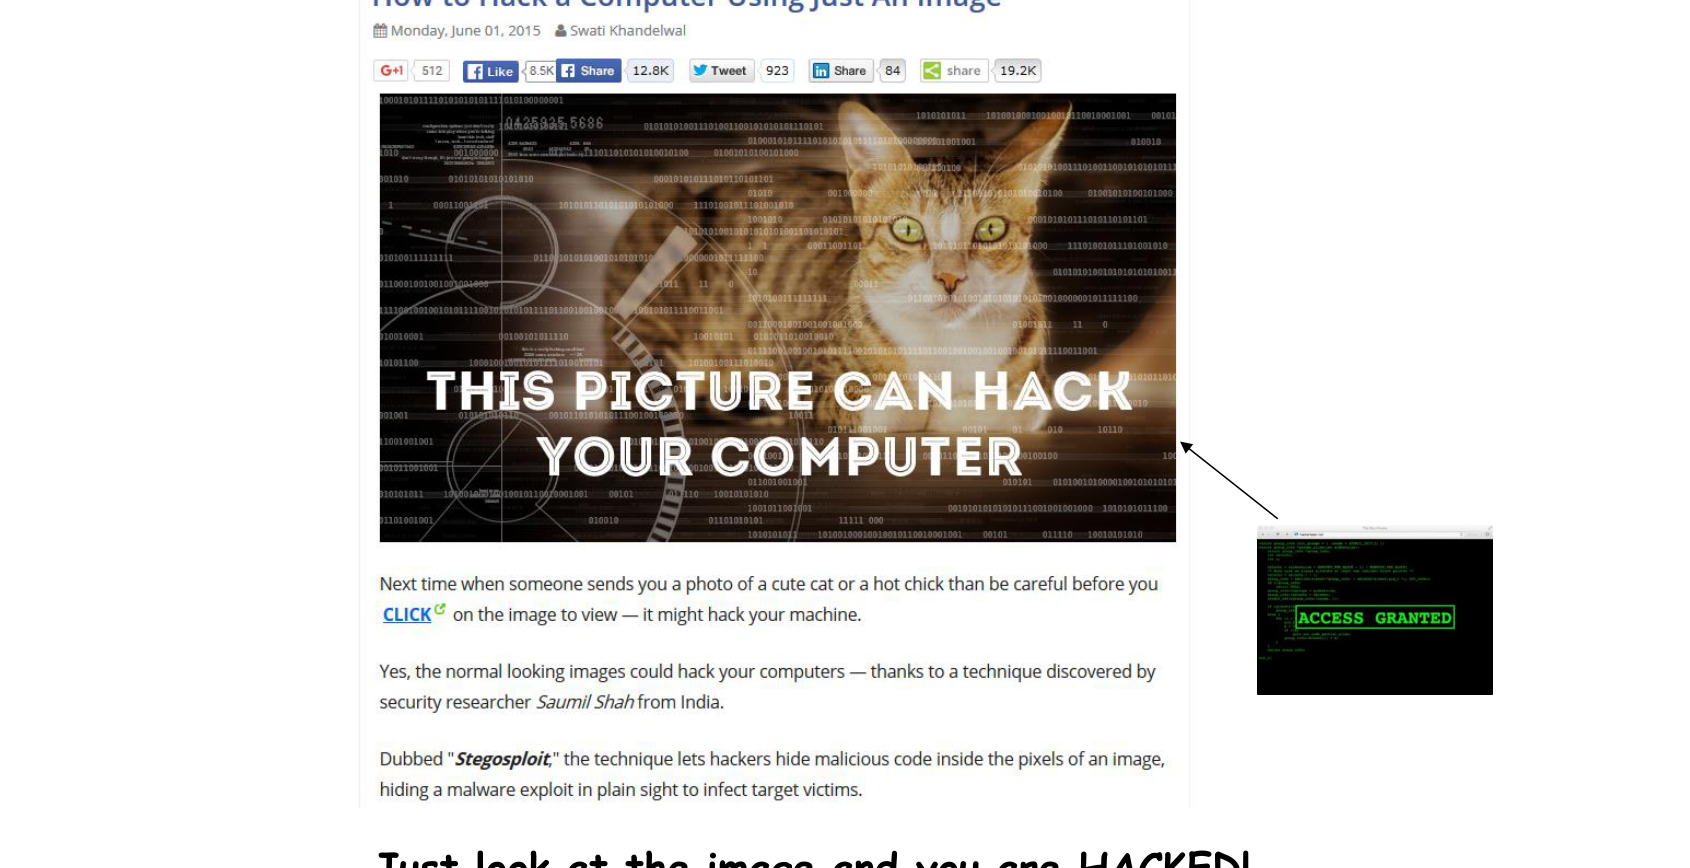
\includegraphics[width=184.80mm,height=238.79mm]{../../images/llm/page_008_img_01.png}%
\end{textblock*}

% deskripsi: Screenshot kecil yang menunjukkan terminal komputer dengan pesan 'ACCESS GRANTED' berwarna hijau.
% bbox normalisasi: [0.7220, 0.5880, 0.8420, 0.7250]
\begin{textblock*}{25.20mm}(151.62mm,174.64mm)
\noindent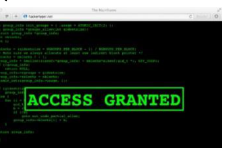
\includegraphics[width=25.20mm,height=40.69mm]{../../images/llm/page_008_img_02.png}%
\end{textblock*}

% bbox perkiraan otomatis: Screenshot artikel berita tentang Stegosploit yang menunjukkan gambar kucing dengan teks overlay 'THIS PICTURE CAN HACK YOUR COMPUTER' dan penjelasan mengenai teknik menyembunyikan kode berbahaya dalam piksel gambar.

\end{document}
